
%(BEGIN_QUESTION)
% Copyright 2006, Tony R. Kuphaldt, released under the Creative Commons Attribution License (v 1.0)
% This means you may do almost anything with this work of mine, so long as you give me proper credit

Since precision pneumatic instruments operate best when their supply air pressure is at a constant pressure, it is necessary to {\it regulate} the fluctuating air pressure from the receiver vessel down to a lower, more constant level for the instrument.  The device designed to do this is called an {\it air pressure regulator}.  A cut-away diagram of an air pressure regulator is shown here:

$$\includegraphics[width=15.5cm]{i00190x01.eps}$$

The wedge-shaped {\it plug} can move down to open the passageway and allow more of the high-pressure air to enter the chamber below the diaphragm, and can move up to close off the passageway and reduce the flow of incoming air into the diaphragm chamber.  The regulation setpoint is adjustable by the position of the threaded rod pressing down on the diaphragm through a spring.

Describe how this air pressure regulator functions.  Suppose that the outlet air pressure is below setpoint.  How does this mechanism respond to bring the outlet pressure back up to where it is supposed to be?  

If the outlet air pressure rises to too high a level, how does the mechanism compensate to reduce it back down to the setpoint level?

\vskip 20pt \vbox{\hrule \hbox{\strut \vrule{} {\bf Suggestions for Socratic discussion} \vrule} \hrule}

\begin{itemize}
\item{} Suppose the spring inside this regulator were to break.  What effect would this have on the regulator's output pressure, and why?
\item{} Suppose the vent hole were to plug.  What effect would this have on the regulator's output pressure, and why?
\end{itemize}

\underbar{file i00190}
%(END_QUESTION)





%(BEGIN_ANSWER)

If the chamber air pressure is too high, the excess pressure will exert more force on the underside of the diaphragm to push it up, thus moving the plug up and closing off the passageway, reducing the air supply flow:

$$\includegraphics[width=15.5cm]{i00190x02.eps}$$

As the outlet air continues to flow out of the regulator, the chamber pressure will eventually drop back down to setpoint, and the passageway will open again.

If the chamber air pressure is too low, the reduced force on the underside of the diaphragm cannot resist the spring force from above, and the plug moves down.  This opens up the passageway, allowing more of the supply air to enter the chamber and increase the pressure:

$$\includegraphics[width=15.5cm]{i00190x03.eps}$$

In short, the opposing forces of spring pressure (and atmospheric air pressure) above the diaphragm, versus the chamber pressure below the diaphragm, act to move the plug up or down as needed to maintain the chamber pressure approximately equal to the equivalent pressure of atmospheric air + spring force on the diaphragm.  

The threaded rod with an attached turn handle adjusts the compression of the spring above the diaphragm, and changes the pressure regulation setpoint.  Screwing the threaded rod in the downward direction will increase the spring force on the top of the diaphragm and likewise increase the equilibrium point between the three forces, increasing the output air pressure regulation setpoint as a consequence.  Screwing the threaded rod in the upward direction will decrease the spring force on the diaphragm's top, decreasing the equilibrium point between the three forces and decreasing the pressure setpoint.

%(END_ANSWER)





%(BEGIN_NOTES)


%INDEX% Basics, pneumatics: pressure regulator

%(END_NOTES)


